\chapter*{2-Mapas de Karnaugh y Algebra de Boole}
\section{Objetivo}
\indent\indent Obtener la representación en mapas de Karnaugh de una función dada. Esta misma debera ser simplifacada aplicando las tecnicas de agrupación vistas en clase. Además se debera realizar mediante el método tradicional del Algebra de Boole.

Finalmente modelaremos el sistema resultante con su correspondiente circuito logico. Luego, dado se expresara este mismo haciendo uso unicamente de compuertas \textit{nand}.

\subsection{Obtención del mapa de Karnaugh}
Dada la siguiente expresión en maxtérminos se pudo interpretar el mapa de Karnaugh de donde provinieron
\[
	f(a,b,c,d)=\prod\left(M_{0},M_{1},M_{5},M_{7},M_{8},M_{10},M_{14},M_{15}\right)
\]
\begin{center}
 \begin{Karnaugh}
 %Inputs are in the order of the max/min termns. Do not use continous inputs. Ex: first term refers to m0/M0, fourth term refers to m2/M2
        \contingut{0,0,1,1,1,0,1,0,0,1,0,1,1,1,0,0}
       	\implicant{2}{6}{red}
       	\implicant{13}{9}{blue}	%Numero de mintermino o Maxtermino
     	\implicant{4}{12}{purple}
     	\implicantdaltbaix[3pt]{3}{11}{green}
    %\implicantcantons[2pt]{orange}
      	%\implicantcostats{3}{11}{green}
    \end{Karnaugh}
\end{center}

Mediante la selección de dichos grupos se obtuvo la siguiente función logica simplificada mediante mintérminos:
\[
	f(a,b,c,d)= b\overline{cd} + a\overline{c}d +
				\overline{b}cd +\overline{a}c\overline{d}
\]

Dado que se han escogido 4 grupos se ha llegado de forma inmediata a dicha formulación

\subsection{Aplicaci\'on del algebra de Boole}
\indent En este apartado desarrollaremos paso por paso las operaciones necesarias para obtener la expresión logica simplificada del sistema dado.
\indent 
Nuestro primer paso es plantear la suma de de los mintérminos:
\[f(a,b,c,d)= \underbrace{\overline{ab}cd}_{m_3}+
			  \underbrace{\overline{ab}c\overline{d}}_{m_2}
			 +\underbrace{\overline{a}b\overline{cd}}_{m_4}
			 +\underbrace{\overline{a}bc\overline{d}}_{m_6}
			 +\underbrace{ab\overline{cd}}_{m_{12}}
			 +\underbrace{ab\overline{c}d}_{m_{13}}
			 +\underbrace{a\overline{bc}d}_{m_9} 
			 +\underbrace{a\overline{b}cd}_{m_{11}}
			 \]
El resultado de su simplificación dependera de cómo se sumen los terminos. 
Primero aplicaremos ciegamente las reglas de simplificación:
\[ 
	f(a,b,c,d)= \underbrace{\overline{ab}c\underbrace{\left(d+ \overline{d}\right)}_{1}}_{m_3 +m_2}
	+
	\underbrace{\overline{a}b\overline{d}\underbrace{\left(c+ \overline{c}\right)}_{1}}_{m_4 +m_6}
	+
	\underbrace{ab\overline{c}\underbrace{\left(d+ \overline{d}\right)}_{1}}_{m_{12} +m_{13}}
	+
	\underbrace{a\overline{b}d\underbrace{\left(c+ \overline{c}\right)}_{1}}_{m_9 +m_{11}}
\]

La expresión simplificada:
\[ 
	f(a,b,c,d)= 
	\overline{ab}c
	+
	\overline{a}b\overline{d}
	+
	ab\overline{c}
	+
	a\overline{b}d
\]


Esta expresión tiene la misma cantidad de terminos que la obtenida mediane el mapa de Karnaugh. 
Ahora se realizara de nuevo la suma pero esta vez se agruparan tal como fueron escogidos los grupos en el mapa.

$$
f(a,b,c,d)= 
\underbrace{\overline{ab}cd + a\overline{b}cd}_{m_3 + m_{11}}
+
\underbrace{\overline{a}b\overline{cd} + ab\overline{cd}}_{m_4+m_{12}}
+
\underbrace{ab\overline{c}d + a\overline{bc}d }_{m_{13} + m_{9}}
+
\underbrace{\overline{ab}c\overline{d} + \overline{a}bc\overline{d}}_{m_2 + m_6}
$$

Simplificando:
$$f(a,b,c,d)= 
\underbrace{\overline{b}cd\underbrace{\left(\overline{a}+a\right)}_{1}}_{m_3 + m_{11}}
+\underbrace{b\overline{cd}\underbrace{\left(\overline{a}+a\right)}_{1}}_{m_4+m_{12}}
+
\underbrace{a\overline{c}d\underbrace{\left(\overline{c}+c\right)}_{1} }_{m_{13} + m_{9}}
+
\underbrace{\overline{a}b\overline{d}\underbrace{\left(\overline{b}+b\right)}_{1}}_{m_2 + m_6}$$


Finalmente, reacomodando los terminos:
\[
	f(a,b,c,d)= b\overline{cd} + a\overline{c}d +
				\overline{b}cd +\overline{a}c\overline{d}
\]

Llegamos nuevamente a la expresión deducida mediane el mapa de 
Karnaugh

\section{Circuito Logico Utilizando compuertas AND,OR y NOT}

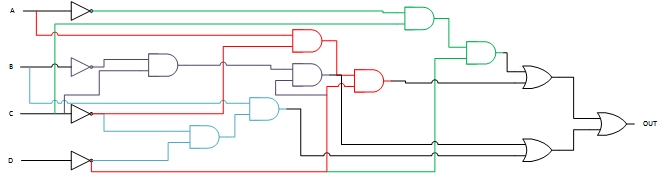
\includegraphics[width=\textwidth]{Ejercicios/Drawing1.jpg}

\section{Circuito Logico Utilizando compuertas NAND}

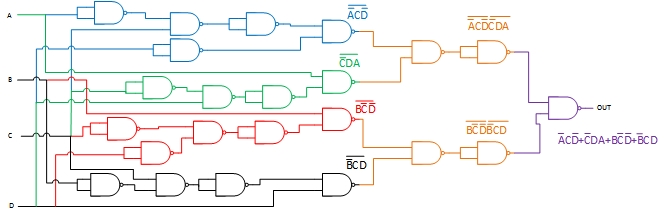
\includegraphics[width=\textwidth]{Ejercicios/circuito2.jpg}
 